%*******************************************************************************
%****************************** Second Chapter *********************************
%*******************************************************************************

\chapter{Rigid Body}
\label{chap:rigid-body}

\ifpdf
    \graphicspath{{Chapter2/Figs/Raster/}{Chapter2/Figs/PDF/}{Chapter2/Figs/}}
\else
    \graphicspath{{Chapter2/Figs/Vector/}{Chapter2/Figs/}}
\fi

In this chapter we introduce the dynamics of a \emph{rigid body}. 
Existing (robot-related) literature on rigid body dynamics can be divided into two main categories. The first category contains work that use almost exclusively \emph{spatial} 6D velocities as defined in Geometrical Mechanics such as \citep{featherstone2008,Featherstone2016,jain2010,murray1994}. The second category include work that use the 6D velocities that are a combination of the ``classical'' linear velocity and the angular velocity of the body \citep{spong2006,siciliano2010robotics,Chiaverini2016}. The connection between these two representations is well known to robotics researcher \citep{murray1994,bruyninckx1996symbolic,englsberger2016}, but it was never explored in depth. Furthermore, it is a common source of confusion for newcomers to the field. In this chapter we treat all the commonly used representation of velocity, explaining the respective advantages and limitations, and the effect of choosing one representation or another on dynamics.

Furthermor, while most robotics textbooks on dynamics introduce the Newton-Euler equations as a given, we prefer to derive them from the basic principle of Lagrangian Dynamics. This methodology is consistent with what is typically done for fixed-based robots \citep{siciliano2010robotics,spong2006}, and is useful to get an insight on the structure of Newton-Euler equations and \emph{why} they are different from the classical Euler-Lagrange equations that describe the evolution of a system whose configuration space is a vector space. 

The goal of this chapter is two-folded: while introducing the kinematics and dynamics of the rigid body, we also introduce a notation for describing kinematics and dynamics 6D quantities,
as well as their coordinate transformations. 

The goal of this newly introduced notation is to be compact, not ambiguous, and in harmony with Lie Group formalism. 
The notation borrows from the well known notation introduced in \citep{featherstone2008}, which is also used, with slight  modifications, in \citep{Featherstone2016}. This notation
is, unfortunately, not fully in accordance with Lie group
formalism used in, e.g., \citep{murray1994,park1995lie,kimlie},
that is, however, less compact than \citep{featherstone2008}, leading to long expressions when several rigid bodies are present. This chapter presents the frames notation, while the connection between the notation and the Lie group formalism is presented in Appendix~\ref{liegroups}.



\section{Overview of the notation}

\begin{remark}
Every chapter will begin with an overview of the notation used in that Chapter. Frequently, the notation used in a given chapter will be a simplified version of the full notation introduced in this chapter, to avoid overloading the text with an extremly complex notation. In some cases, the simplified notation can only be introduced for a single section. In that case, an overview of the simplified notation used in that section will open the section.
\end{remark}

\[
  \left[
      \begin{tabular}{@{\quad}m{.05\textwidth}@{\quad}m{.83\textwidth}}
        {\Huge \faInfoCircle} &
          \raggedright%
          \textbf{Notation used through the thesis} \par
          \begin{tabular}{@{}p{0.18\textwidth}p{0.60\textwidth}@{}}
          $A$,$B$        & coordinate frames \\
$p$            & an arbitrary point \\
$o_B$          & origin of $B$ \\
$[A]$          & orientation frame associated to $A$ \\
$B[A]$         & frame with origin $o_B$ 
                 and orientation $[A]$ \\
$\ls^Ap$       & coordinates of $p$ 
                 w.r.t. to $A$ \\
$\ls^Ao_B$     & coordinates of $o_B$ w.r.t. to $A$ \\
$\ls^AH_B$     & homogeneous transformation from $B$ to $A$ \\
$\ls^AX_B$     & velocity transformation 
                 from $B$ to $A$  \\
$\ls^C\rmv_{A,B}$ & 6D velocity expressing the velocity of $B$ wrt to $A$
                 written in $C$ \\
$\ls^C\rmv_{A,B}^\wedge$ 
               & $4\times4$ matrix representation of
                 $\ls^C\rmv_{A,B}$\\
$\ls^C\rmv_{A,B}\times$
               & $6\times6$ matrix representation of 
                 the 6D velocity cross product \\
$\ls^C\rmv_{A,B}\bts$
               & $6\times6$ matrix representation of 
                 the dual cross product \\
$\ls_B\rmf$       & coordinates of the 6D force $\rmf$
                 w.r.t. $B$ \\
$\ls_AX^B$     & 6D force transformation 
                 from $B$ to $A$ \\
$\left<\ls_B\rmf, \ls^B\rmv_{A,B}\right>$
               & pairing between 6D force and velocity \\
$\ls_B\bbM_L$  & $6\times6$ inertia tensor of link (=rigid body) $L$\\ & expressed with respect to frame $B$ \\
          \end{tabular}
      \end{tabular}
    \right]
\]



% $\ls^CJ_{A,B}$ & Jacobian relating the velocity of
% $B$ with respect to $A$ expressed in $C$ \\
% $\ls^CJ_{A,B/F}$ & Jacobian relating the velocity of
% $B$ with respect to $A$ expressed in $C$, \\ & where
% the floating base velocity is expressed in $F$\\

\section{Math preliminaries}
The following notation is used throughout the thesis.
\begin{itemize}

\item
The set of real numbers is denoted by $\mathbb{R}$. 
Let $u$ and $v$ be two $n$-dimensional column vectors of real numbers, i.e. $u,v \in \mathbb{R}^n$, 
then their inner product is denoted as $u^T v$, with ``$T$'' the transpose operator. 

\item
The identity matrix of dimension~$n$ is denoted
$I_n \in \mathbb{R}^{n \times n}$; the zero column vector of dimension~$n$ is denoted $0_n \in \mathbb{R}^n$; the zero matrix of dimension~$n \times m$ is denoted $0_{n \times m} \in \mathbb{R}^{n \times m}$.

\item
The set $\SO(3)$ is
the set of $\mathbb{R}^{3 \times 3}$ orthogonal matrices with determinant equal to one, namely
\begin{align}
\SO(3) :=  \{\, R \in \mathbb{R}^{3 \times 3} \mid R^T R = I_3 , \hspace{0.3em} \operatorname{det}(R) = 1 \,\}.
\end{align}
% When endowed with matrix multiplication, $\SO(3)$ becomes a Lie group, the {\em Special Orthogonal} group of dimension three.

\item The set $\so(3)$, read {\em little} $\so(3)$, is
the set of $3 \times 3$ skew-symmetric matrices, 
\begin{align}
\so(3) :=  \{\, S \in \mathbb{R}^{3 \times 3}  \mid S^T = -S \,\}.
\end{align}
% When endowed with the matrix commutator as operation, 
% the set becomes a Lie algebra.

\item The set $\SE(3)$ is defined as
\begin{align}
\SE(3) :=  
\Big\{ 
\begin{bmatrix} R & p \\ 0_{1\times3} & 1 \end{bmatrix} \in \mathbb{R}^{4 \times 4} \mid 
R \in \SO(3), p \in \mathbb{R}^3
\Big\} .
\end{align}
% When endowed with matrix multiplication, it becames
% the \emph{Special Euclidean} group of dimension three, a Lie group that can be used to represent rigid transformations and their composition in the 3D space.
\item The set $\se(3)$ is defined as
\begin{align}
\se(3) :=  
\Big\{ 
\begin{bmatrix} \Omega & v \\ 0_{1\times3} & 0 \end{bmatrix} \in \mathbb{R}^{4 \times 4}  \mid \Omega \in \so(3), v \in \mathbb{R}^3 
\Big\}.
\end{align}
% When endowed with the matrix commutator as operation,
% $\se(3)$ becomes the Lie algebra of the Lie group $\SE(3)$.


% \marginpar{\tiny AS: Somewhere in the text
%we have to explain that the hat operator represents 
%{\em both} the Lie algebra homeomorphism between $\mathbb{R}^3$ and $\so(3)$ and the matrix representation of $\mathbb{R}^3$ to itself.
% Sometimes this Lie algebra is indicated as $\mathbb{R}^3_\times = (\mathbb{R}^3, \times)$.
% }
\item Given the vector $w = (x; y; z) \in \mathbb{R}^3$, 
we define $w^\wedge$ (read $w$ {\em hat}) as the $3\times3$ \emph{skew-symmetric} matrix 
\begin{equation}\label{eq:hat3}
w^\wedge = 
\begin{bmatrix} 
 x \\ 
 y \\
 z 
\end{bmatrix}^{\wedge}
:=
\begin{bmatrix}
  \phm 0   & -z     & \phm y \\
  \phm z   & \phm 0 & -x     \\
      -y   & \phm x & \phm 0 
\end{bmatrix} \in \so(3).
\end{equation}
Given the \emph{skew-symmetric matrix} $W = w^\wedge$, 
we define $W^\vee \in \mathbb{R}^3$ (read $W$ {\em vee}) as
\begin{equation}
W^{\vee} = 
\begin{bmatrix}
  \phm 0   & -z     & \phm y \\
  \phm z   & \phm 0 & -x     \\
      -y   & \phm x & \phm 0 
\end{bmatrix}^{\vee}
:=
\begin{bmatrix} 
 x \\ 
 y \\
 z 
\end{bmatrix}
\in \mathbb{R}^3 .
\end{equation}
Clearly, the vee operator is the inverse of the hat operator. 



\item 
Given a vector $\rmv = ( v; \omega ) \in \mathbb{R}^6$, 
$v$ and $\omega \in \mathbb{R}^3$, we define
\begin{align}\label{eq:hat6}
  \rmv^{\wedge} 
  =
 \begin{bmatrix}
  v \\
  \omega
  \end{bmatrix}
  ^{\wedge} 
& :=
  \begin{bmatrix} 
    \omega^\wedge & v \\
    0_{1\times3}  & 0 
  \end{bmatrix} \in \se(3).
\end{align}

\item
Similarly to what was done for vectors in $\mathbb{R}^3$ few lines above, 
we define the vee operator as the inverse of the hat operator such that
\begin{align}
\begin{bmatrix}
  \omega^\wedge  & v \\ 
  0_{1\times3}        & 0 
\end{bmatrix}^{\vee}
:=
\begin{bmatrix}
  v \\
  \omega
\end{bmatrix}  
= \rmv \in \mathbb{R}^6.
\end{align}

\item Given $A \in \mathbb{R}^{n \times m}$ and $B \in \mathbb{R}^{p \times q}$, we denote with $\otimes$ the Kronecker product $A \otimes B \in \mathbb{R}^{np \times mq}$.
\item Given $X \in \mathbb{R}^{m \times p}$, $\text{vec}(X) \in \mathbb{R}^{nm}$ denotes the column vector obtained by stacking the columns of the matrix~$X$. 
In view of the definition of $\text{vec}(\cdot)$, it follows that \begin{equation}\label{eq:kroneckerVec} \text{vec}(AXB) = \left( B^{\top} \otimes A \right) \text{vec}(X).\end{equation}

\begin{comment}
 \item
 Given two normed vector spaces $E$ and $F$ and a function between them $f : E \mapsto F$ we define as the derivative of $f$ in $x_0 \in E$ as the linear function $D f(x_0) : E \mapsto F$ such that:
 \begin{align}
    \lim_{x \to x_0} \frac{||f(x)-f(x_0) -  Df(x_0)\cdot(x-x_0)||}{||x-x_0||} = 0
 \end{align}
\marginpar{\tiny\color{red}AS: Silvio, not sure to you have the right equations after (9), but you are clearly pointed in the right direction. In general, I like calling the perturbation $z$}
If $E = \mathbb{R}$ and $F = \mathbb{R}$ then $D f(x_0)$ is the linear function tangent to $f(x)$, that is usually indicated as:
$$
 D f(x_0)\cdot x= \left.\frac{d f}{d x}\right|_{x=x_0} (x-x_0) + f(x_0) .
 $$
If $E = \mathbb{R}^n$ and $F = \mathbb{R}^m$ then  %$D f(x_0)$ is:
$$
D f(x_0)\cdot x = 
\begin{bmatrix} 
\frac{\partial f_1}{\partial x_1} & \frac{\partial f_1}{\partial x_2} & \hdots & \frac{\partial f_1}{\partial x_n} \\ 
\frac{\partial f_2}{\partial x_1} & \frac{\partial f_2}{\partial x_2} & \hdots & \frac{\partial f_2}{\partial x_n} \\ 
\vdots & \vdots & \ddots & \vdots                    \\ 
\frac{\partial f_m}{\partial x_1} & \frac{\partial f_m}{\partial x_2} & \hdots & \frac{\partial f_m}{\partial x_n} 
\end{bmatrix}_{x = x_0}
(x-x_0) + f(x_0) .
$$

Given a function $f$ of $p$ normed vector spaces $f : E_1 \times E_2 \hdots E_p \mapsto F$ we define as $D_1 f$ the derivative of $f$ with respect to $E_1$, with $D_2 f$ the derivative of $f$ with respect to $E_2$ and so on so forth. 

We refer to \cite[Chapter 2]{spivak1965calculus} and to \cite[Section 2.3]{abraham2012manifolds} for further details on the derivative notation ($D$, $D_1$, $D_2$, $\dots$) used in this document.
\end{comment}

\end{itemize}

\section{Frame kinematics}

\subsection{Rigid Body Assumption}
\label{sec:rigidBodyAssumption}
A rigid body is an idealization of a physical object, in which the deformation internal to the object are assumed to be negligible, i.e. the object is assumed to be \emph{nondeformable}. While in the real physical world every object that is interacting with the external world is subject to a certain degree of deformation, in the study of certain mechanism such a humanoid robots, the rigid body assumption is useful as it permits to develop model that capture the \emph{dominant dynamics} of the analyzed system, disregarding any aspect related to the internal compression and decompression of the object composing the system. 


The kinematics of a rigid body are typically described by attaching to the rigid body a {\em frame}, defined as the combination of a point (called  {\em origin}) and an {\em orientation frame} in the 3D space \citep{DeLaet2013,spong2006}. For this reason in this section
we will describe the kinematics of frames, and this will serve also for describing the kinematics of any rigid body.

\subsection{Points and coordinate frames}

We typically employ 
a capital letter to indicate a frame. Given a frame $A$, we will indicate with $o_A$ its origin and with $[A]$ its orientation frame.
Formally, we write this as $A = (o_A, [A])$.

Frames can be time varying. They can be used, e.g., to describe the position and orientation in space of a rigid body as time evolves.
They are also used to expressed a coordinate system for a 6D force exchanged by two bodies
or used to define a coordinate system
to describe a robot task (like a frame attached to the center of mass and oriented as the inertial frame). 

Newton's mechanics defines the set of \emph{Inertial} frames. In this document, we usually indicate one inertial frame as \ with $A$ (the \emph{A}bsolute frame). As common practice, for robots operating near the Earth surface, we will assume the frame $A$ to be fixed to the world's surface, disregarding non-inertial effects due to the Earth's motion.

\subsubsection{Coordinate vector of a point}
Given a point $p$, its coordinates with respect to a frame $A = (o_A, [A])$ are collected in the {\em coordinate vector} ${~\!\!}^A p$. The coordinate vector ${~\!\!}^A p$ represents the coordinates of the 3D geometric vector ${\overset{\rightarrow}{r}}_{o_A,p}$ connecting the origin of frame $A$ with the point $p$, pointing towards $p$, expressed in the orientation frame $[A]$,
that is
\begin{align}
  ~^A p 
& := 
  \begin{bmatrix}
  {\overset{\rightarrow}{r}}_{o_A,p} 
  \cdot 
  {\overset{\rightarrow}{x}}_A \\
  {\overset{\rightarrow}{r}}_{o_A,p} 
  \cdot 
  {\overset{\rightarrow}{y}}_A \\
  {\overset{\rightarrow}{r}}_{o_A,p} 
  \cdot 
  {\overset{\rightarrow}{z}}_A
  \end{bmatrix}
\in \mathbb{R}^3,
\end{align}
with $\cdot$ denoting the scalar product
between two vectors and
${\overset{\rightarrow}{x}}_A$,
${\overset{\rightarrow}{y}}_A$,
${\overset{\rightarrow}{z}}_A$,
the unit vectors defining
the orientation frame $[A]$.

\subsubsection{Change of orientation frame}
Given two frames $A$ and $B$, we will employ the notation
\begin{equation}
  \ls^{A} R_{B} \in \SO(3) 
\end{equation}
to denote the coordinate transformation from frame $B$ to frame $A$. 
The coordinate transformation $\ls^A R_B$ only depends on the
relative orientation between the orientation frames $[A]$ and $[B]$,
irrespectively of the position of the origins $o_A$ and $o_B$. 

\subsubsection{Homogeneous transformation}
To describe the position and orientation of a frame $B$ with respect to another frame $A$, we employ the $4\times4$ homogeneous matrix
\begin{equation}
  \label{eq:homogeneousTransformation}
  \ls^A H_B :=
     \begin{bmatrix}
     \ls^A R_B & \ls^A o_B \\
     0_{1\times3} & 1
  \end{bmatrix} .
\end{equation}
Given a point $p$, the homogeneous transformation matrix $\ls^A H_B$ can be also used to map the coordinate vector $\ls^A p$ to $\ls^B p$ as follows. Let 
$\ls^A \bar p$ and $\ls^B \bar p$ denote the {\em homogenous representation} of $\ls^A p$ and $\ls^B p$, respectively. That is, let
$\ls^A \bar p := (\ls^A p; 1) \in \mathbb{R}^4$ and likewise for
$\ls^B \bar p$ (note that ; indicates row concatenation). Then
\begin{align} \label{eq:Abp_AHB_Bbp}
  \ls^A \bar p 
& = 
  \ls^A H_B \ls^B \bar p ,
\end{align}
which is the matrix form of 
$\ls^A p = \ls^A R_B \ls^B p + \ls^A o_B$. We refer the interested readers to \citep[Chapter 2]{murray1994} for further details on homogeneous representation of rigid transformations. 

\subsection{6D Velocity vectors} 
In the following, given a point $p$ and
a frame $A$, we define
\begin{align}
\label{eq:Adotp}
  \ls^A \dot p :=  \frac{d}{dt} \left( \ls^A p \right) .
\end{align}
In particular, when $p$ is the origin of a frame, e.g., $p = o_B$, we have
$$
 \ls^A \dot{o}_B =
 \frac{d}{dt} \left(\ls^A o_B \right) .
$$
It is important to note that, by itself, expressions like $\dot o_B$ or $\dot p$ have {\em no} meaning.
Similarly to \eqref{eq:Adotp}, we also define
\begin{align}
\ls^{A} \dot{R}_{B} & := \frac{d}{dt} \left( ~^{A} R_{B} \right) \\
\intertext{and} 
  \ls^A \dot H_B 
  & := \frac{d}{dt} \left( \ls^A H_B \right)
   = 
  \begin{bmatrix}
    \ls^A {\dot R}_B & \ls^A {\dot o}_B \\
     0_{1\times3} & 0
  \end{bmatrix} .
\end{align}
The relative velocity between a frame $B$ with respect to a frame $A$ can be represented by the time derivative of the homogenous matrix 
$\ls^A H_B \in \SE(3)$. A more \emph{compact} representation of 
$\ls^A {\dot H}_B$ can be obtained
multiplying it by the inverse of $\ls^A H_B$ on the left or on the right.
In both cases, the result is an element of the $\se(3)$ that will be called 
a {\em 6D velocity}. Premultipliying on the left, one obtains
\begin{align} \label{eq:se3ex}
  \ls^{A} H_{B}^{-1} \ls^{A} \dot{H}_{B}  
  & =  
  \begin{bmatrix} 
    \ls^A {R}_B^T & -\ls^A {R}_B^T \ls^Ao_B \\
    0_{1\times3} & 1
  \end{bmatrix}
  \begin{bmatrix}
    \ls^A \dot{R}_B & \ls^A{\dot o}_B \\
    0_{1\times3} & 0
  \end{bmatrix} 
  \notag\\
  & =
  \begin{bmatrix}
    \ls^AR_B^T \ls^A {\dot R}_B & \ls^AR_B^T \ls^A {\dot o}_B \\
    0_{1\times3} & 0
  \end{bmatrix} .
\end{align}
Note that $\ls^A {R}_B^T \ls^A \dot{R}_B$ appearing on the right hand side of \eqref{eq:se3ex} is skew symmetric. 
Define $\ls^B v_{A,B}$ and $\ls^B \omega_{A,B} \in \mathbb{R}^3$ so that
\begin{align}
\label{eq:BvAB}
  \ls^B v_{A,B} 
& := 
  \ls^A R_B^T \ls^A {\dot o}_B ,
\\ 
\label{eq:BwAB}
  \ls^B \omega^{\wedge}_{A,B} 
& := 
  \ls^A R_B^T \ls^A {\dot R}_B .
\end{align}
The \emph{left trivialized} velocity of frame $B$ 
with respect to frame $A$ is
\begin{equation}
\ls^B \rmv_{A,B} := 
\begin{bmatrix}
\ls^{B} v_{A,B} \\
\ls^{B} \omega_{A,B}
\end{bmatrix} 
\in \mathbb{R}^6 .
\end{equation}
By construction, 
\begin{align}\label{eq:defBVAB}
  \ls^B \rmv^{\wedge}_{A,B} 
& = 
  \ls^{A} H_{B}^{-1}  \ls^{A} \dot{H}_{B} .
\end{align}
Note the slight abuse of notation in using the
hat operator $\wedge$ in \eqref{eq:BwAB}
and \eqref{eq:defBVAB} that maps a vector
into its corresponding matrix representation 
(respectively, from $\R^3$ to $\R^{3\times 3}$
using \eqref{eq:hat3} in \eqref{eq:BwAB} and from $\R^6$ to $\R^{4\times4}$ using \eqref{eq:hat6} in \eqref{eq:defBVAB}).

% This 6D velocity can have represented as a 4x4 matrix with the \emph{left trivialization}:
% \begin{eqnarray}
%  ~^B \rmv_{A,B}^\wedge & = ~^{B} H_{A}  ~^{A} \dot{H}_{B} = \\ 
%    &\begin{bmatrix}
%    ~^{B}  {R}_{A}   & ~^B o_A \\
%     0_{1\times3} & 1
%  \end{bmatrix}   
%     \begin{bmatrix}
%    ~^{A} \dot{R}_{B}   &   ~^A 
%    \dot{o}_B \\
%     0_{1\times3} & 0
%  \end{bmatrix} = \\
%  &\begin{bmatrix}
%    ~^{B}  {R}_{A} ~^{A} \dot{R}_{B}   & ~^{B}  {R}_{A} {}^{A} \dot{o}_B \\
%     0_{1\times3} & 0
%  \end{bmatrix} = \\
%  & \begin{bmatrix} 
%    (~^{B} \omega_{A,B})^\wedge & 
%    ~^{B} v_{A,B} \\ 
%    0_{1\times3} & 0 
%    \end{bmatrix}
%\end{eqnarray}

\noindent 
Specularly to what was done in \eqref{eq:se3ex}, 
right multiplying $\ls^A {\dot H}_B$ by the inverse of
$\ls^A H_B$ leads to
\begin{align}
  \ls^A {\dot H}_B  \ls^A H_B^{-1} 
& =  
  \begin{bmatrix}
    \ls^{A} \dot{R}_{B}   & \ls^A {\dot o}_B \\
     0_{1\times3} & 0
  \end{bmatrix}
  \begin{bmatrix} 
    \ls^A R_B^T & -\ls^A R_B^T \ls^A o_B \\
    0_{1\times3} & 1
  \end{bmatrix}
\notag\\
& =
  \begin{bmatrix}
     \ls^{A} \dot{R}_{B}  \ls^A R_B^T & 
          \ls^A {\dot o}_B - \ls^{A} \dot{R}_{B} \ls^A R_B^T \ls^A o_B \\
     0_{1\times3} & 0
  \end{bmatrix} .
\end{align}
Define
$\ls^A v_{A,B}$ and $\ls^A \omega_{A,B} \in \mathbb{R}^3$ 
as
\begin{align}
\label{eq:AvAB}
  \ls^A v_{A,B} 
& := 
  \ls^A {\dot o}_B - \ls^{A} \dot{R}_{B} \ls^A R_B^T \ls^A o_B
\\
\label{eq:AwAB}
  \ls^A \omega^{\wedge}_{A,B} 
& := 
  \ls^{A} \dot{R}_{B}  \ls^A R_B^T.
\end{align}
The \emph{right trivialized} velocity of $B$ with respect to $A$ is then defined as
\begin{equation}
\ls^A \rmv_{A,B} := 
\begin{bmatrix}
\ls^{A} v_{A,B} \\
\ls^{A} \omega_{A,B}
\end{bmatrix} 
\in \mathbb{R}^6 .
\end{equation}
By construction, 
\begin{align} \label{eq:defAVAB}
  \ls^A \rmv^{\wedge}_{A,B} 
& = 
  \ls^{A} \dot{H}_{B} \ls^{A} H_{B}^{-1} .
\end{align}

The \emph{right trivialized} and \emph{left trivialized} representation of the velocity between two frames are general concepts, that can be applied to any pair of frames in the 3D space. When the frame $A$ is an inertial frame and the $B$ frame is rigidly attached to a body, as we will assume in this chapter, these velocities representations are also called \emph{inertial velocity} and \emph{body velocity}.

The mapping between $\ls^A \rmv_{A,B}$ and  $\ls^B \rmv_{A,B}$ is trivial to express in matrix form, as it follows directly from their definitions that:
$$
\ls^A \rmv_{A,B}^\wedge = \ls^A H_B \ls^B \rmv_{A,B}^\wedge \ls^A H_B^{-1}
$$
From this expression, it is clear that the ``frame transformation'' mapping between $\ls^B \rmv_{A,B}$ and  $\ls^A \rmv_{A,B}$ is a linear mapping. By writing the 6D velocity in linear form:
$$
\ls^A \rmv_{A,B} = \ls^A X_B \ls^B \rmv_{A,B} 
$$

with:
\begin{equation}
\label{eq:adjTransform}
\ls^A X_B = \ls^A X_B \left( \ls^A H_B \right) = 
\begin{bmatrix}
\ls^A R_B &  \ls^A o_B^\wedge \ls^A R_B \\
0_{3 \times 3} & \ls^A R_B .
\end{bmatrix}
\end{equation}

This is usually called the \emph{adjoint} matrix.

\begin{remark}
\label{rem:dotNotation}
Through out this thesis, given a quantity such as position, velocity, etc., we define the \emph{dot operator} $\dot{(-)}$  as the total time derivative of the quantity. Hence, given a 6D velocity $\ls^C \rmv$ expressed in a frame $C$, the symbol $\ls^C \dot{\rmv}$ means
\begin{equation*}
\ls^C \dot{\rmv} = \frac{d}{dt}\left(\ls^C\rmv\right).
\end{equation*}
While this may be obvious and pedantic, let us recall that the  \emph{ dot operator} $\dot{(-)}$ is defined differently in some of the robotics dynamics literature. For instance, given a 6D velocity $\ls^C \rmv$ expressed in a frame $C$, \cite[Section 2.10]{featherstone2008} defines $\ls^C \dot{\rmv}$ as
\begin{equation*}
    \ls^C X_A \frac{d}{dt}(\ls^A \rmv),
\end{equation*}
where $A$ is an arbitrary (and often hidden) inertial frame with respect to (w.r.t.) which the derivative is computed.
\end{remark}

\todo[inline]{Insert mapping to lie group theory of adjoint representations}

\subsection{Adjoint matrix as a change of frame} 
The $6 \times 6$ transform is ubiquous in multibody dynamics, and it is usually interpreted as the ``change of frame'' in which the frame velocity is expressed. 
 Let's assume that we have a frame $\tilde{B}$ that is rigidly attached to the frame $B$, i.e. : 
\begin{equation}
    \ls^B \dot{H}_{\tilde{B}} = 0
\end{equation}
Noting that $\ls^A H_{\tilde{B}} = \ls^A H_{B} \ls^B H_{\tilde{B}}, \ls^A \dot{H}_{\tilde{B}} = \ls^A \dot{H}_{B} \ls^B H_{\tilde{B}}$, we can see that the mapping between the left-trivialized velocity of frame $B$ and the left trivialized velocity of frame $\tilde{B}$ is given by:
\begin{IEEEeqnarray}{rCl}
\ls^{\tilde{B}} \rmv_{A,\tilde{B}}^\wedge &=& \ls^A H_{\tilde{B}}^{-1} \ls^A \dot{H}_{\tilde{B}} = \\
&=& \ls^B H_{\tilde{B}}^{-1} \ls^{B} \rmv_{A,B}^\wedge \ls^B H_{\tilde{B}}.
\end{IEEEeqnarray}
From which we have: 
$$
\ls^{\tilde{B}} \rmv_{A,\tilde{B}} = \ls^{\tilde{B}} \rmv_{A,{B}} = \ls^{\tilde{B}} X_B \ls^B \rmv_{A,B} .
$$

Similarly, if we imagine to define a new frame $\tilde{A}$ rigidly attached to our previous frame $A$, we will have: 
\begin{equation}
    \ls^{\tilde{A}} \rmv_{A,B} = \ls^{\tilde{A}} X_A \ls^A \rmv_{A,B} .
\end{equation}

This gives us a nice ``interpretation'' of the linear component of the left-trivialized velocity as the velocity of the origin of a frame fixed to the frame $B$ that is instantaneously coincident with the frame $A$, that has been popularized by \citep{featherstone2008}.


\subsubsection{Mixed velocity}
In the previous subsection we introduce the left-trivialized and right-trivialized velocity of a frame $B$ with respect to an frame $A$. In the next chapter we will further discuss their use and properties, but for the moment we want to highlight a ``peculiar'' feature of both this velocities representation: in neither cases the linear part of the velocity is the derivative of the position vector of the origin of the frame $B$, i.e. $\ls^A \dot{o}_B$ . On the other hand, it is quite common for undergraduate physics textbooks or even in robotics \citep{siciliano2010robotics} to represent the velocity of a rigid body as a 6D vector given by:
\begin{equation}
\begin{bmatrix}
   \ls^A \dot{o}_B \\
   \ls^A \omega_{A,B}
\end{bmatrix}
\end{equation}
To simplify the description of the algorithms and concepts available in this thesis, we need a way to express this quantity coherently with the rest of the concepts introduced until know.

Fortunately this can be easily interpreted as a left or right trivialized velocity associated with the appropriate change of frame. In particularly, we introduce the frame $B[A] := (o_B,[A])$, that is, the frame
with the same origin of $B$ and same
orientation of $A$. We have then:
\begin{equation}
    \ls^{B[A]} H_B = 
    \begin{bmatrix}
     \ls^A R_B & 0_{3 \times 1} \\
      0_{1 \times 3} & 1 
    \end{bmatrix},
\end{equation}
and by expressing the velocity $\rmv_{A,B}$ in $B[A]$, we get:
\begin{equation}\label{eq:B[A]VAB}
  \ls^{B[A]} \rmv_{A,B} = 
  \ls^{B[A]}X_B \ls^B \rmv_{A,B} = 
   \begin{bmatrix} ~^{A} {R}_{B} & 0 \\ 0 &  ~^{A} {R}_{B}  \end{bmatrix} \begin{bmatrix} ~^{B} {R}_{A} {}^{A} \dot{o}_B \\ {}^B \omega_{A,B}  \end{bmatrix} 
   = \begin{bmatrix} \ls^A \dot{o}_B \\ \ls^A \omega_{A,B} \end{bmatrix}.
\end{equation}
In \citep{bruyninckx1996symbolic,murray1994,englsberger2016}, \eqref{eq:B[A]VAB} is referred to as the \emph{hybrid} velocity of frame $B$ with respect to frame $A$.
To avoid confusion with hybrid systems theory, we will call
\eqref{eq:B[A]VAB} the {\em mixed velocity} 
of frame $B$ with respect to frame $A$ ({\em mixed} as it has both the flavors of a left trivialized velocity for the linear velocity part and of a right trivialized velocity for
the angular velocity part).

Table~\ref{tab:velRecap} collects the definitions of the different representation of the 6D velocity, and the conversion formulas to convert one representation into another.

\todo[inline]{Explain how the different representation depend on the rotation and position part of the representation (i.e. all depend on the rotation w.r.t of the inertial, but just the inertial depend on the position part.}

\section{Frame acceleration}
The acceleration of a frame (attached to a rigid body) is a quantity for which the definition is far from being obvious, as already noted in literature \citep{Featherstone2001}. Before introducing the representation for a rigid body acceleration most used in literature, and their properties, we will discuss the cross product for 6D velocities, a useful operator to study the properties of the different accelerations.

\subsection{The cross product on $\mathbb{R}^6$ ($\times$)}
Equation \eqref{eq:defBVAB} can be rewritten as
\begin{align}
  \ls^A{\dot H}_B & = 
  \ls^AH_B \ls^B\rmv_{A,B}^\wedge .
\end{align}
By time differentiation of \eqref{eq:adjTransform}, it can be shown that
a similar formula holds for $\ls^AX_B$, namely, that
\begin{align} \label{eq:dAXBdt}
  \ls^A{\dot X}_B & = 
  \ls^AX_B \ls^B\rmv_{A,B}\times
\end{align}
with $\ls^B\rmv_{A,B}\times$ defined as
\begin{equation}
\label{eq:defBVABcross}
\ls^B\rmv_{A,B} \times := 
\begin{bmatrix}
\ls^B\omega_{A,B}^\wedge & 
\ls^Bv_{A,B}^\wedge \\
0_{3 \times 3} & 
\ls^B\omega_{A,B}^\wedge
\end{bmatrix}.
\end{equation}
We will refer to \eqref{eq:defBVABcross} as
the matrix representation 
of the {\em cross product on $\mathbb{R}^6$}. 

\begin{remark}
The connection between the cross product on $\R^6$ introduced here and its equivalent concepts in the Lie group language is discussed in the appendix, in particular in Subsection~\ref{subsec:crossProductAndLieGroups}.
\end{remark}



\subsubsection{Basic properties of the cross product}

Equation \eqref{eq:defBVABcross} defines a cross product between vectors of $\mathbb{R}^6$, with the classical anticommutative property
\begin{equation}
\ls^C\rmv_{A,B}\times \ls^C\rmv_{D,E}
=
-\ls^C\rmv_{D,E}\times\ls^C\rmv_{A,B} .
\end{equation}
As a direct consequence of anticommutativity is 
\begin{equation}
\label{eq:autoCrossIsNull}
\ls^C\rmv_{A,B} \times \ls^C\rmv_{A,B} = 0_{6 \times 1}.
\end{equation}
% At deeper look at the cross product defined via \eqref{eq:defBVABcross} reveals that this operation turns
% $\mathbb{R}^6$ into a Lie algebra, a vector space with a anticommutative bilinear operation satisfying the Jacobi identity
% \cite[Chapter 9]{marsden1999introduction}.

\subsection{Acceleration representations and their relation}
By direct derivation with respect to time of the left-trivialized, right-trivialized and mixed 6D velocity, we obtain the respective accelerations, that are described in detail in Table~\ref{tab:accRecap}. All the conversions between the accelerations are also detailed in Table~\ref{tab:accRecap}, and make an extensive use of the 6D cross product introduced in this section. Please remember that the definition of the dot notaton $\dot{(\cdot)}$ is clarified in Remark~\ref{rem:dotNotation}.

In the case that the frame $A$ is an inertial frame, some alternative representation of the acceleration between a frame $B$ and the inertial frame $A$ are used in literature, that are described hereafter.
\subsection{``Sensor'' acceleration}
We define the ``sensor'' acceleration as:
\begin{equation}
    \alpha_{A,B} = \ls^B X_{B[A]} \ls^{B[A]} \dot{\rmv}_{A,B} 
    = 
    \begin{bmatrix}
   \ls^B R_A \ls^A \ddot{o}_B \\
   \ls^B \dot{\omega}_{A,B}
\end{bmatrix}
\end{equation}
This acceleration is used for example in \citep{siciliano2010robotics}. Its relationship with inertial sensing will be discussed in Subsection~\ref{subsec:linkSensors}. 

\begin{sidewaystable}
\small
\begin{tabular}{|c | c | c | c | m{2cm} | c |} 
 \hline
 Name & Symbol & Definition & Left-Trivialized & Right-Trivialized & Mixed \\ [0.5ex] 
 \hline
 Left-Trivialized & 
 $\ls^B \rmv_{A,B}$ & 
 $\begin{bmatrix} 
 \ls^A R_B^T \ls^A {\dot o}_B \\
 \left( \ls^A R_B^T \ls^A {\dot R}_B \right)^{\vee}
 \end{bmatrix}$ &
 $\ls^B \rmv_{A,B}$ & 
 $\ls^B X_A \ls^A \rmv_{A,B}$ & 
 $\ls^B X_{B[A]} \ls^{B[A]} \rmv_{A,B}$ \\
 \hline
 Right-Trivialized & 
 $\ls^A \rmv_{A,B}$ & 
 $\begin{bmatrix} 
 \ls^A {\dot o}_B - \ls^{A} \dot{R}_{B} \ls^A R_B^T \ls^A o_B \\
 \left( \ls^A {\dot R}_B \ls^A R_B^T \right)^{\vee}
 \end{bmatrix}$ &
 $\ls^A X_B \ls^B \rmv_{A,B}$ & 
 $\ls^A \rmv_{A,B}$ & 
 $\ls^A X_{B[A]} \ls^{B[A]} \rmv_{A,B}$ \\
 \hline
 Mixed & 
 $\ls^{B[A]} \rmv_{A,B}$ & 
 $\begin{bmatrix} 
 \ls^A {\dot o}_B \\
 \left( \ls^A {\dot R}_B \ls^A R_B^T  \right)^{\vee}
 \end{bmatrix}$ &
 $\ls^{B[A]} X_B \ls^B \rmv_{A,B}$ & 
 $\ls^{B[A]} X_A \ls^A \rmv_{A,B}$ & 
 $\ls^{B[A]} \rmv_{A,B}$ \\
 \hline
\end{tabular}
\caption{Conversion rules between the different representations of frame 6D velocity.}
\label{tab:velRecap}

\bigskip\bigskip

 \begin{tabular}{|c | c | c | c | c|} 
 \hline
  $=$ & 
  $\ls^B \dot{\rmv}_{A,B}$ &
  $\ls^A \dot{\rmv}_{A,B}$ &
  $\ls^{B[A]} \dot{\rmv}_{A,B}$ &
  $\alpha$ 
  \\ [0.5ex] 
 \hline
 $\ls^B \dot{\rmv}_{A,B}$ & 
 $\ls^B \dot{\rmv}_{A,B}$ & 
 $\ls^B X_A \ls^A \dot{\rmv}_{A,B}$ & 
 $\ls^B X_{B[A]} \ls^{B[A]} \dot{\rmv}_{A,B} - 
 \begin{bsmallmatrix}
\left( \ls^B R_A \ls^A  \dot{o}_B \right) \times \ls^B \omega_{A,B} \\ 
 0_{3 \times 1} 
 \end{bsmallmatrix} $ & 
 $\alpha 
 - 
 \begin{bsmallmatrix}
 \left( \ls^B R_A \ls^A \dot{o}_B \right) \times \ls^B \omega_{A,B}  \\ 
 0_{3 \times 1} 
 \end{bsmallmatrix}
 $ 
 \\
 \hline
  $\ls^A \dot{\rmv}_{A,B}$ & 
  $\ls^A X_B \ls^B \dot{\rmv}_{A,B}$ & 
  $\ls^A \dot{\rmv}_{A,B}$ & 
  $\ls^A X_{B[A]} \ls^{B[A]} \dot{\rmv}_{A,B} - 
 \begin{bsmallmatrix}
 \ls^A  \dot{o}_B \times \ls^A \omega_{A,B} \\ 
 0_{3 \times 1} 
 \end{bsmallmatrix}$  & 
  $\ls^A X_{B} \alpha - 
 \begin{bsmallmatrix}
 \ls^A  \dot{o}_B \times \ls^A \omega_{A,B} \\ 
 0_{3 \times 1} 
 \end{bsmallmatrix}$
 \\
 \hline
 $\ls^{B[A]} \dot{\rmv}_{A,B}$ & 
 $
 \ls^{B[A]} X_B  \ls^B \dot{\rmv}_{A,B}
 +\begin{bsmallmatrix}
 \ls^A  \dot{o}_B \times \ls^A \omega_{A,B} \\ 
 0_{3 \times 1} 
 \end{bsmallmatrix}$
  & 
  $
  \ls^{B[A]} X_A  \ls^A \dot{\rmv}_{A,B}
  +\begin{bsmallmatrix}
 \ls^A  \dot{o}_B \times \ls^A \omega_{A,B} \\ 
 0_{3 \times 1} 
 \end{bsmallmatrix}$ & 
$\ls^{B[A]} \dot{\rmv}_{A,B}$ & 
 $\ls^{B[A]} X_{B} \alpha \ $
 \\
 \hline  
 $\alpha$ & 
  $
  \ls^B \dot{\rmv}_{A,B}
  +
  \begin{bsmallmatrix}
 \left( \ls^B R_A \ls^A \dot{o}_B \right) \times \ls^B \omega_{A,B}  \\ 
 0_{3 \times 1} 
 \end{bsmallmatrix}$ & 
    $
    \ls^B X_A \ls^A \dot{\rmv}_{A,B}
  +
  \begin{bsmallmatrix}
 \left( \ls^B R_A \ls^A \dot{o}_B \right) \times \ls^B \omega_{A,B}  \\ 
 0_{3 \times 1} 
 \end{bsmallmatrix}$ & 
  $\ls^{B} X_{B[A]} \ls^{B[A]} \dot{\rmv}_{A,B} $ & 
 $\alpha$ \\
 \hline
\end{tabular}
\caption{Conversion rules between the different representations of frame 6D acceleration.}
\label{tab:accRecap}
\end{sidewaystable}

\subsection{``Proper'' acceleration}
\label{subsec:properAcceleration}
It is widespread, in the literature on multibody dynamics applied to robotics, to sometimes refer to a vector of the acceleration minus the gravitational acceleration. 
The same symbols is sometime used to refer both to the acceleration with respect earth-fixed inertial frame and this acceleration minus gravity. To avoid confusion, in this thesis we will always refer to this as \emph{proper acceleration}, as opposed to the \emph{coordinate acceleration}, consistently with the nomenclature used in relativity theory \citep{fraundorf1996}.

We define first the ``proper'' acceleration using the ``sensor'' representation, as: 
\begin{equation}
\label{eq:properSensorAcc}
\alpha^g_{A,B} := \alpha_{A,B} - 
\begin{bmatrix} \ls^B R_A \ls^A g  \\
 0_{3 \times 1}
\end{bmatrix}
\end{equation}
Note that this is the acceleration that can be obtained by an inertial measurement unit aligned with $B$, as the linear part of it is the output of a linear accelerometer, and the angular part is the derivative of the output of a gyroscope. This is thoroughly discussed in Section~\ref{subsec:accelerometer}. 

For all other accelerations, we define: 
\begin{IEEEeqnarray}{rCl}
\IEEEyesnumber
\ls^{B} \rma^g &:=& \ls^B \dot{\rmv} - \begin{bmatrix} \ls^B R_A \ls^A g \\ 0_{3 \times 1} \end{bmatrix}, \IEEEyessubnumber \\
\ls^{A} \rma^g &:=& \ls^A \dot{\rmv} - \begin{bmatrix} \ls^A g \\ 0_{3 \times 1} \end{bmatrix}, \IEEEyessubnumber \\
\ls^{B[A]} \rma^g &:=& \ls^{B[A]} \dot{\rmv} - \begin{bmatrix} \ls^A g \\ 0_{3 \times 1} \end{bmatrix} \IEEEyesnumber
\end{IEEEeqnarray}
as respectively the \emph{left-trivialized}, \emph{right-trivialized} and \emph{mixed} proper acceleration. Note that all the conversion rules presented in Table~\ref{tab:accRecap} still hold for proper acceleration in the presented form. 

\subsection{Illustrative Example: the Spinning Wheel}
\begin{figure}
\begin{tikzpicture}
\node[inner sep=0pt] (floatingBase) at (0,0) {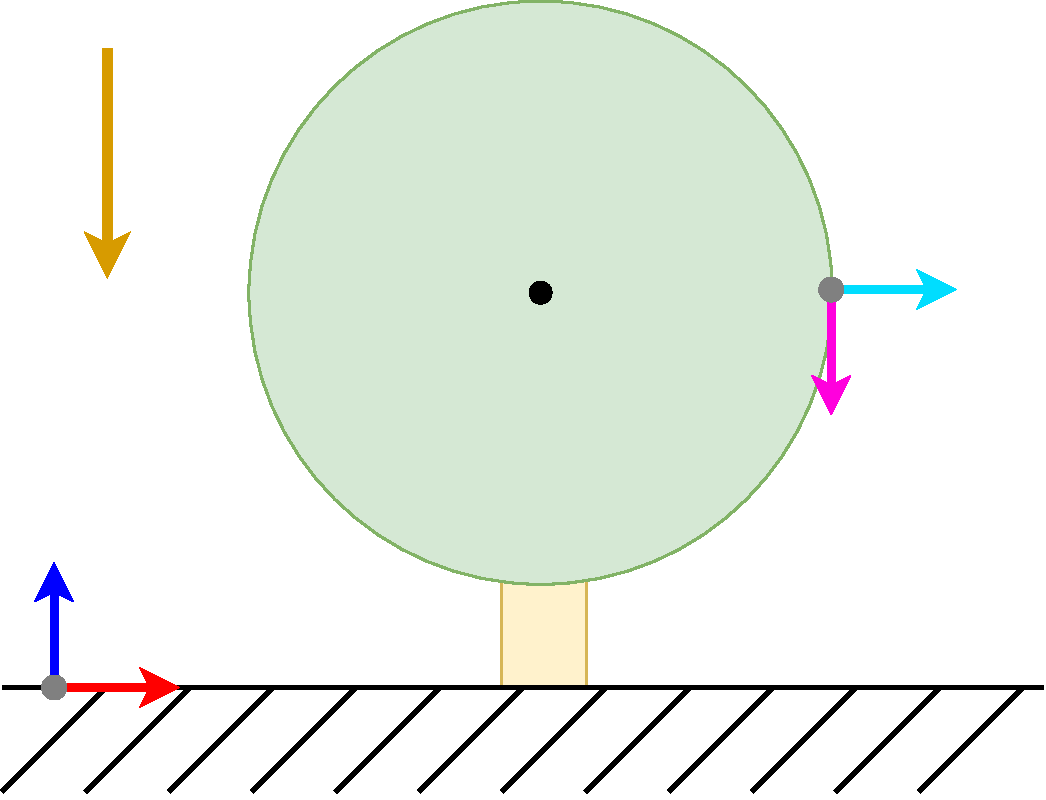
\includegraphics[width=\linewidth]{Figs/velocityAndAccelerationGraphs.pdf}};
\node[inner sep=0pt] (A) at (-5,-3.1) {\Large $A$};
\node[inner sep=0pt] (g) at (-4.5,3.2) {\Large $g$};
\node[inner sep=0pt] (B) at (3.2,0.3) {\Large $B$};
\draw [->,thick,black,line width=1pt] (0.15,2.0) arc (90:0:0.8);
\node[inner sep=0pt] (theta) at (1.0,1.8) {\Large $\theta$};
\node[inner sep=0pt] (oC) at (0.0,1.0) {\Large $o_C$};
\end{tikzpicture}
\caption{Spinning wheel, with the gravity acceleration $g$, the inertial frame $A$ and the moving frame $B$ at $\theta = -\frac{\pi}{2}$.}
\label{fig:spinningWheel}
\end{figure}


To see a concrete example of the definition just presented, we use a spinning wheel, depicted in Figure~\ref{fig:spinningWheel}. An inertial frame $A$ is rigidly attached to the ground, while there is a moving frame $B$ attached to the external part of a wheel of radius $r$ spinning around the axis:
$$\ls^A a = \ls^B a =  \begin{bmatrix} 0 \\ 0 \\ 1 \end{bmatrix}$$
passing in the point $o_C$. Furthermore, the system is affected by a uniform gravitational field with the gravity acceleration vector, whose expression in the $A$ orientation is:
$$\ls^A g = \begin{bmatrix} 0 \\ - |g| \\ 0 \end{bmatrix}.$$ 
The location of the spinning wheel w.r.t. the inertial frame is given by the angle $\theta$. Assuming that for $\theta = 0$ the orientation of $A$ and $B$ coincide, we can define the transform between $A$ and $B$ as (where we define $H := \ls^A H_B$ and $R := \ls^A R_B$ to avoid overloading the notation).

\begin{IEEEeqnarray}{rClrCl}
H(\theta) &=&  
\begin{bmatrix}
R(\theta) & 
\ls^A o_C + 
R(\theta) 
\begin{bsmallmatrix}
0 \\ r \\ 0
\end{bsmallmatrix} \\
0_{1 \times 3} & 1 
\end{bmatrix}, \hspace{0.5em}
R(\theta) &=& 
\begin{bmatrix}
\cos(\theta) & - \sin(\theta) & 0 \\
\sin(\theta) & \cos(\theta) & 0 \\
0 & 0 & 1 
\end{bmatrix}.
\end{IEEEeqnarray}

Taking the derivatives w.r.t. to time, we have that:
\begin{IEEEeqnarray*}{rClrCl}
\dot{H}(\theta,\dot{\theta}) &=&  
\begin{bmatrix}
\dot{R}(\theta,\dot{\theta})  & 
\dot{R}(\theta,\dot{\theta}) 
\begin{bsmallmatrix}
0 \\ r \\ 0
\end{bsmallmatrix}
\\ 
0_{1 \times 3} & 0
\end{bmatrix}, 
\\
\dot{R}(\theta,\dot{\theta}) &=& 
\begin{bmatrix}
-\sin(\theta) & -\cos(\theta) & 0 \\
\cos(\theta) & -\sin(\theta) & 0 \\
0 & 0 & 0 
\end{bmatrix} \dot{\theta},
\\
R^T(\theta) \dot{R}(\theta) &=& 
\begin{bmatrix}
0 & -1 & 0 \\
1 & 0 & 0 \\
0 & 0 & 0 
\end{bmatrix} \dot{\theta},
\\
\dot{R}(\theta) R^T(\theta) &=& 
\begin{bmatrix}
0 & -1 & 0 \\
1 & 0 & 0 \\
0 & 0 & 0 
\end{bmatrix} \dot{\theta}.
\end{IEEEeqnarray*}

Using the definition of left-trivialized, right-trivialized and mixed velocity summarized in Table~\ref{tab:velRecap} we then have:
\begin{IEEEeqnarray*}{rCCCl}
\ls^B \rmv_{A,B} &=&  
\begin{bmatrix}
\ls^B v_{A,B} \\
\ls^B \omega_{A,B}
\end{bmatrix}
=
\begin{bmatrix}
R^T \ls^A \dot{o}_B \\
(R^T \dot{R})^\vee
\end{bmatrix}
&=& 
\begin{bmatrix}
- r  \\
0 \\
0 \\
0 \\
0 \\
1
\end{bmatrix} \dot{\theta},
\\ 
%%%%%%
% RIGHT-TRIVIALIZED VELOCITY
%%%%%%
\ls^A \rmv_{A,B} &=& 
\begin{bmatrix}
\ls^A v_{A,B} \\
\ls^A \omega_{A,B}
\end{bmatrix}
=
\begin{bmatrix} 
 \ls^A {\dot o}_B -\dot{R} R^T \ls^A o_B \\
 \left( {\dot R} R^T \right)^{\vee}
 \end{bmatrix}
 &=&
 \begin{bmatrix}
 \begin{bmatrix}
 -\cos(\theta)  r \\
 -\sin(\theta)  r \\
0 
 \end{bmatrix}
 - {\begin{bmatrix} 0 \\ 0 \\ 1 \end{bmatrix}  }^\wedge \ls^A o_B

\\
0 \\
0 \\
1 
\end{bmatrix}
\dot{\theta} 
,
\\
\ls^{B[A]} \rmv_{A,B} &=&
\begin{bmatrix}
\ls^{B[A]} v_{A,B} \\
\ls^{B[A]} \omega_{A,B}
\end{bmatrix}
=
\begin{bmatrix} 
 \ls^A {\dot o}_B \\
 \left( {\dot R} R^T \right)^{\vee}
 \end{bmatrix}
 &=&
\begin{bmatrix}
 -\cos(\theta) r \\
-\sin(\theta)  r  \\
0 \\
0 \\
0 \\
1
\end{bmatrix}
\dot{\theta} 
+ 
.
\end{IEEEeqnarray*}
Similarly, for the accelerations defined in Table~\ref{tab:accRecap} we then have:
\begin{IEEEeqnarray*}{rCl}
%%%%%%
% LEFT-TRIVIALIZED ACCELERATION
%%%%%%
\ls^B \dot{\rmv}_{A,B} &=&
\begin{bmatrix}
- r  \\
0 \\
0 \\
0 \\
0 \\
1
\end{bmatrix} \ddot{\theta}
\\
%%%%%%
% RIGHT-TRIVIALIZED ACCELERATION
%%%%%%
\ls^A \dot{\rmv}_{A,B}
 &=&
 \begin{bmatrix}
 \begin{bmatrix}
 -\cos(\theta)  r \\
 -\sin(\theta)  r \\
0 
 \end{bmatrix}
 - {\begin{bmatrix} 0 \\ 0 \\ 1 \end{bmatrix}  }^\wedge \ls^A o_B

\\
0 \\
0 \\
1 
\end{bmatrix}
\ddot{\theta}
+
\begin{bmatrix}
  \begin{bmatrix}
     \sin(\theta)  r \\
     -\cos(\theta)  r \\
     0 
  \end{bmatrix} 
  - 
  {\begin{bmatrix} 0 \\ 0 \\ 1 \end{bmatrix}  }^\wedge 
    \begin{bmatrix}
     -\cos(\theta)  r \\
     -\sin(\theta)  r \\
     0 
  \end{bmatrix} 

\\
0 \\
0 \\
0 
\end{bmatrix}
\dot{\theta}^2
,\\
%%%%%%
% MIXED ACCELERATION
%%%%%%
\ls^{B[A]} \dot{\rmv}_{A,B} &=&
\begin{bmatrix}
 -\cos(\theta) r \\
-\sin(\theta)  r  \\
0 \\
0 \\
0 \\
1
\end{bmatrix}
\ddot{\theta} 
+
\begin{bmatrix}
 \sin(\theta) r \\
-\cos(\theta)  r  \\
0 \\
0 \\
0 \\
0
\end{bmatrix}
\dot{\theta}^2 
,\\
%%%%%%
% SENSOR-TRIVIALIZED ACCELERATION
%%%%%%
\alpha_{A,B} &=& 
\begin{bmatrix}
-r \\
0  \\
0 \\
0 \\
0 \\
1
\end{bmatrix}
\ddot{\theta} 
+
\begin{bmatrix}
0\\
-r  \\
0 \\
0 \\
0 \\
0
\end{bmatrix}
\dot{\theta}^2 
= 
\begin{bmatrix}
-r \ddot{\theta} \\
-r \dot{\theta}^2   \\
0 \\
0 \\
0 \\
\ddot{\theta} 
\end{bmatrix}
.
\end{IEEEeqnarray*}

\begin{comment}
\subsection{Transforming absolute velocities and accelerations}
We not discuss how this transforms are modified if a new inertial frame $\tilde{A}$ or a new body frame $\tilde{B}$ is chosen to represent velocity or accelerations. 
Please note that by definition of body frame, $\tilde{B}$ needs to be rigidly attached to the old body frame $B$. On the other hand, in theory it is perfectly fine for two inertial frames to have a relative linear velocity between them, but for the sake of simplicity we will also assume that $\tilde{A}$ and $A$ are rigidly attached. 

\subsubsection{Change of ``'' frame}
\begin{IEEEeqnarray}{rCl}
\ls^B \rmv_{\tilde{A},B} &=& \ls^B \rmv_{A,B} \\
\ls^{\tilde{A}} \rmv_{\tilde{A},B} &=& \ls^{\tilde{A}} X_A \ls^A \rmv_{A,B} \\
\ls^{B[\tilde{A}]} \rmv_{\tilde{A},B} &=& \ls^{B[\tilde{A}]} X_{B[A]} \ls^{B[A]} \rmv_{A,B}
\end{IEEEeqnarray}

\begin{IEEEeqnarray}{rCl}
\ls^B \dot{\rmv}_{\tilde{A},B} &=& \ls^B \dot{\rmv}_{A,B} \\
\ls^{\tilde{A}} \dot{\rmv}_{\tilde{A},B} &=& \ls^{\tilde{A}} X_A \ls^A \dot{\rmv}_{A,B} \\
\ls^{B[\tilde{A}]} \dot{\rmv}_{\tilde{A},B} &=& \ls^{B[\tilde{A}]} X_{B[A]} \ls^{B[A]} \dot{\rmv}_{A,B} \\
\alpha_{\tilde{A},B} = \alpha_{\tilde{A},B}
\end{IEEEeqnarray}

\subsubsection{Change of body frame}
\begin{IEEEeqnarray}{rCl}
\ls^{B^{'}} \rmv_{A,B^{'}} &=& \ls^{B^{'}} X_B \ls^B  \rmv_{A,B} \\
\ls^{A} \rmv_{A,\tilde{B}} &=& \ls^A \rmv_{A,B} \\
\ls^{\tilde{B}[A]} \rmv_{A,\tilde{B}} &=& \ls^{\tilde{B}[A]} X_{B[A]} \ls^{B[A]} \rmv_{A,B}
\end{IEEEeqnarray}

\begin{IEEEeqnarray*}{rCl}
\IEEEyesnumber
\ls^{\tilde{B}} 
\dot{\rmv}_{A,\tilde{B}} 
&=& 
\ls^{\tilde{B}} X_B \ls^B \dot{\rmv}_{A,B}, \IEEEyessubnumber \\ 
\ls^{A} \dot{\rmv}_{A,\tilde{B}} &=& \ls^A \dot{\rmv}_{A,B}, \IEEEyessubnumber \\
\ls^{\tilde{B}[A]} \dot{\rmv}_{A,\tilde{B}} &=& \ls^{\tilde{B}[A]} X_{B[A]} \ls^{B[A]} \dot{\rmv}_{A,B} 
+ \IEEEnosubnumber \\
 &+& \ls^{\tilde{B}[A]} X_{B[A]} \ls^{B[A]} \rmv_{\tilde{B}[A],B[A]} \times \ls^{B[A]} \rmv_{A,B}, \IEEEyessubnumber \\ 
\alpha_{A,\tilde{B}} &=& \ls^{\tilde{B}} X_{B} \left( \alpha_{A,B} + \ls^{B} \rmv_{\tilde{B}[A],B[A]} \times \ls^{B} \rmv_{A,B} \right). \IEEEyessubnumber
\end{IEEEeqnarray*}
For a greater insight, we recll that $\ls^{B[A]} \rmv_{\tilde{B}[A],B[A]} = \begin{bmatrix} \ls^A \omega_{A,B}^\wedge \ls^A R_{\tilde{B}} \ls^{\tilde{B}} o_B \\ 0_{3 \times 1}  \end{bmatrix} $ and $\ls^{B} \rmv_{\tilde{B}[A],B[A]} = \begin{bmatrix} \ls^B \omega_{A,B}^\wedge \ls^B R_{\tilde{B}} \ls^{\tilde{B}} o_B \\ 0_{3 \times 1}  \end{bmatrix} $.
\end{comment}

\section{Force-Torque covectors}

In classical mechanics, the interaction between a rigid body and the enviroment is described by \emph{interaction} forces. 
While this forces can be described as a system of forces acting on finite number of contact points 
% or as a \emph{distribution} of forces acting on the contact surface, 
it is common to represent the effect of this interaction forces as a 6D force-torque vector, in which the first three elements are the sum of all the contact forces, while the last three coordinate are the sum of the moments of this forces with respect to a given point in space. Similarly to the 6D velocity case, also for the 6D force-torque can be said to be represented in different frames, in which the \emph{origin} of the frame is the point with respect to which the moment is taken and the \emph{orientation} is the one in which the forces and moments are expressed. In particular we indicate the coordinates of a 6D force $\rmf$ 
with respect to frame $B$ with
\begin{equation}
\ls_B\rmf := 
\begin{bmatrix}
\ls_Bf \\
\ls_B\tau
\end{bmatrix} \in \R^6. 
\end{equation}
Note that the frame $B$ is simply used to indicate the coordinate frame with respect to which the 6D force $\rmf$ is expressed in coordinates and there is no necessity for the 6D force $\rmf$ to also be applied to, e.g., the rigid body (if any) to which $B$ is attached. Similarly to what we did for a 6D velocities, we can define a linear map to change the coordinates of a 6D force from a frame $B$ to another frame $A$. This coordinate transformation is indicated with $\ls_AX^B$ and written as
\begin{align}
  \ls_A\rmf = \ls_AX^B \ls_B\rmf . 
\end{align}
The mapping $\ls_AX^B$ is actually induced by the velocity transformation \eqref{eq:adjTransform} (why this is the case will be explained below) and is related to $\ls^BX^A$ via the definition
\begin{equation} \label{eq:defBXAstar}
  \ls_AX^B := \ls^BX^T_A .
\end{equation}
It is important to realize that \eqref{eq:defBXAstar} is such to make the following identity (of power) hold
\begin{align}
\left<\ls_B \rmf, \ls^B\rmv_{A,B} \right> = 
\left<\ls_A \rmf, \ls^A\rmv_{A,B} \right> ,
\end{align}
where $\rmf$ can be interpreted as a 6D force applied to a rigid body to which the moving frame $B$ is rigidly attached and $A$ as the absolute inertial frame.
\\

\subsection{The dual cross product on $\R^6$ ($\bts$)}

The time derivative of the 6D force coordinate transformation $\ls_A X^B$ has an expression that is dual to velocity coordinate transformation $\ls^AX_B$ given in \eqref{eq:dAXBdt}. Indeed, straightforward computations lead to obtain
\begin{align}\label{eq:dBXAstardt}
  \ls_A{\dot X}^B 
  & = 
  \ls_A X^B \ls^B \rmv_{A,B} \bts 
\end{align}
where the (matrix representation of the) dual cross product $\bts$ is defined by 
\begin{align} \label{eq:defBVABbts}
\ls^B\rmv_{A,B} \bar\times^* :=
\begin{bmatrix}
\ls^B\omega_{A,B}^\wedge & 
0_{3 \times 3} \\
\ls^Bv_{A,B}^\wedge & 
\ls^B\omega_{A,B}^\wedge
\end{bmatrix}.
\end{align}
It is worth noting that \eqref{eq:defBVABbts}
is obtained from \eqref{eq:defBVABcross} by simply transposing this latter expression and taking the negative value of the result: a fact that is also encoded in the symbol $\bts$, where 
the overline sign has been chosen to represent the minus sign and the star the transpose operation (more formally, the adjoint of a linear map, typically indicated with a star). 
The dual cross product \eqref{eq:defBVABbts}
takes one 6D velocity and one 6D force and return one 6D force (as opposed to the cross product \eqref{eq:defBVABcross} that takes as input two 6D velocity and return one 6D velocity); this is also the reason why the sub- and superscripts in  \eqref{eq:dBXAstardt} makes sense:
when $\ls_A{\dot X}^B$ is applied to a 
6D force $\ls_B\rmf$ expressed in $B$, the dual cross product between $\ls^B \rmv_{A,B}$ and the 6D force will return a 6D force expressed in $B$ that can then be converted into a 6D force expressed in $A$ via $\ls_AX^B$. It is also straighforward to prove that
\begin{align}
\ls_A X^B \ls^B \rmv_{A,B} \bts 
& = 
\ls^A \rmv_{A,B} \bts \ls_A X^B .
\end{align}

\begin{remark}
The connection between the cross product on $\R^6$ introduced here and its equivalent concepts in the Lie group language is discussed in the appendix, in particular in Subsection~\ref{subsec:dualCrossProductAndLieGroups}.
\end{remark}

\section{Rigid Body Dynamics}
\label{sec:rigidBodyDynamics}

To discuss rigid body dynamics, we tipically only are interested in two frames: an inertial frame $A$ and a body-fixed frame $B$. To avoid confusion in the readers, throughout this section we then use a simplified notation, summarized in the next notation table.  
\[
  \left[
      \begin{tabular}{@{\quad}m{.05\textwidth}@{\quad}m{.83\textwidth}}
        {\Huge \faInfoCircle} &
          \raggedright%
          \textbf{Simplified Notation, valid for  Section~\ref{sec:rigidBodyDynamics}} \par
          \begin{tabular}{@{}p{0.24\textwidth}p{0.55\textwidth}@{}}
               $A$ & Inertial frame. \\
               $B$ & Frame rigidly attached to the body. \\
               $o := \ls^A o_B$ & Origin of the body w.r.t. to the inertial frame. \\         
               $R := \ls^A R_B$ & Rotation of the body w.r.t. to the inertial frame. \\
               $H := \ls^A H_B$ & Pose of the body w.r.t. to the inertial frame. \\
               $\rmv = \begin{bmatrix} v \\ \omega \end{bmatrix} := \ls^B \rmv_{A,B} $ & Left-trivialized velocity of the body.  \\
               $p := \ls^A p$ & Generic point of the body expressed in the inertial frame $A$. \\
               $r := \ls^B p$ & Generic point of the body expressed in the body frame $B$. \\
               $\rho(\cdot)$ & Density function, taking in input points expressed in the body frame $B$. 
          \end{tabular}
      \end{tabular}
    \right]
\]

\begin{comment}
The first derivation of the dynamics of an unconstrained rigid body can be found in \citep{euler1776}, the 
work that introduced the concept of rigid body itself. In this section we will derive this equation from the least action principle, using Euler-\Poincare equations. 
\end{comment}

All the results of system in classical mechanics can be obtained by applying the principle of least action, that states that the trajectories of a mechanical systems are the extremum of a trajectory-dependent quantity called \emph{action}.

\begin{comment}
With respect to the classical application of this principles, the main difference with rigid body dynamics is that the state $g$ is an element of a (Matrix) Lie Group. While in general the least action principle can be shown to be equivalent to the Euler-Lagrange equations, the Lie-Group based Least Action Principle is equivalent to the Euler-\Poincare equations, as explained in detailed in the Appendix~\ref{liegroups}, in particular in Theorem~\ref{thm:leastActionPrincipleForLieGroups}. 

Using the principle of least action enunciated in Theorem~
\ref{thm:leastActionPrincipleForLieGroups} we can just look into obtaining the \emph{Action}. In view of of \eqref{eq:variational} the Action of a rigid body is uniquely defined by its Lagrangian $L(H,\dot{H})$. One just needs to find a (tractable) version of such lagrangian to obtain the equation of motions of the rigid body.
The lagrangian of the rigid body is given by the difference between the kinetic energy and the potential energy: 
$$
L = T - U .
$$
\end{comment}

\subsection{Review of Lagrangian Dynamics: the point mass}
Before approaching the lagrangian dynamics of the rigid body, we review the basic concepts of lagrangian mechanics using a simple example, a point mass.

The configuration of a point mass with respect to an inertial frame $A$ is given by its position coordinate vector $\ls^A p \in \R^3$. To avoid overloading the notation, in the remainder of this subsection we will indicate the position of the point mass simply as $p := \ls^A p \in \R^3$. The velocity of the point mass is given by the derivative w.r.t to time of the point position, i.e. $\dot{p} := \ls^A \dot{p}$. 

Assuming that the point mass lies in a uniform gravitational field, and the effect of the point mass on the gravitational field is negligible, the Lagrangian for a point mass $m$ is the difference between the Kinetic Energy $K(p,\dot{p})$ and the Potential (Gravitational) Energy $U(p)$:
\begin{IEEEeqnarray}{rCl}
\label{eq:pointMassLagrangian}
\IEEEyesnumber
L(p,\dot{p}) &=& K(p,\dot{p}) - U(p), \IEEEyessubnumber
\\
K(p,\dot{p}) &=& \frac{1}{2} m \left| \dot{p}  \right|^2,  \IEEEyessubnumber \\
U(p) &=& m g^Tp. \IEEEyessubnumber
\end{IEEEeqnarray}

where $g \in \R^3$ is the gravitational acceleration vector of the uniform field.

The action of a given trajectory is defined as:
$$
S[p(\cdot)] = \int_{t_0}^{t_1} L(p(t),\dot{p}(t)) dt 
$$

The Principle of Least Action states that the trajectory performed by such a system is the one that minimize the action. Such a variational problem can be demonstrated to have the same solution of the Euler-Lagrange differential equations \citep{bullo2005}:
$$
\frac{\partial}{\partial p} L(p,\dot{p}) - \frac{d}{dt} \frac{\partial}{\partial \dot{p}} L(p,\dot{p}) = 0 .
$$

In the point mass case we have:
\begin{IEEEeqnarray}{rCl}
\frac{\partial}{\partial p} L(p,\dot{p}) &=& \frac{\partial}{\partial p} U(p) = mg , \IEEEyessubnumber \\
\frac{\partial}{\partial \dot{p}} L(p,\dot{p}) &=& \frac{\partial}{\partial \dot{p}} K(p,\dot{p}) = m\dot{p} , \IEEEyessubnumber \\
\frac{d}{dt} \frac{\partial}{\partial \dot{p}} L(p,\dot{p}) &=& m \ddot{p} . \IEEEyessubnumber
\end{IEEEeqnarray}

From which we have: 
\begin{equation}
m \ddot{p} - m g = 0_{3 \times 1} .
\end{equation}

The left term of the equations is $0$ only if the only external force acting on the point mass is the gravitational force described by the potential $U(p)$. If forces not described by the potential are acting on the point mass, the equation is modified to include this forces acting on the point:
\begin{equation}
m \ddot{p} - m g = f .
\end{equation}

\subsection{Rigid Body Lagrangian Dynamics}
In the previous subsection we reviewed the Lagrangian Dynamics formalism and the principle of Least Action for a simple point mass. In this section we will see how the same concepts applies, with the appropriate changes, to the Rigid Body case. But first we need to formally introduce the concept of \emph{rigid body}, that was informally presented in Section~\ref{sec:rigidBodyAssumption}.

\begin{definition}[Rigid Body]
A \emph{rigid body} is a mathematical abstraction describing an arbitrary distribution of mass in the 3D space, that is fixed with respect to a given frame, that we call the \emph{body} frame $B$. 
\end{definition}

\begin{definition}[Volumetric Mass Density]
The mass distribution of a rigid body in space is described by a time-invariant \emph{density function}, that maps each 3D point (expressed in the frame $B$) to its \emph{density}. 
\begin{equation}
\rho(\cdot): \mathbb{R}^3 \mapsto \mathbb{R}_{\ge 0} .
\end{equation}

The mass $m(V)$ enclosed in a given 3D volume $V$ is given by the \emph{integral} of the density over such a volume:
\begin{equation} 
m(V) = \iiint_{V} \rho\left( r \right) \, dr . 
\end{equation}
\end{definition}

Note that if the density domain was defined as the points in the 3D space expressed in the \emph{inertial} $A$ frame, the density function would have not been constant, but it would also explicitly depend on time. As the density of the rigid body is constant in the body frame $B$, the pose of the \emph{rigid body} can be fully represented by the homogeneous transformation between the \emph{body} frame $B$ and the \emph{inertial frame} $A$, that for simplicity in this section we will indicate as $H = \ls^A H_B$, with $R = \ls^A R_B$ and $o = \ls^A o_B$.

The relation between a point attached to the rigid body expressed in the absolute frame $\ls^A p$, that for simplicity we refer as $p$ and in the body frame $\ls^B p$ (for simplicity $r$) is simply given as:
\begin{equation}
\begin{bmatrix}
  p \\
  1
\end{bmatrix}
= 
\begin{bmatrix}
  R & o \\
  0_{1\times3} & 1 
\end{bmatrix}
\begin{bmatrix}
  r \\
  1
\end{bmatrix}
= 
\begin{bmatrix}
R r + o \\ 
1
\end{bmatrix}
\end{equation}

And its velocity is obtained as:
\begin{equation}
\begin{bmatrix}
  \dot{p} \\
  0
\end{bmatrix}
= 
\begin{bmatrix}
  \dot{R}& \dot{o} \\
  0_{1\times3} & 0 
\end{bmatrix}
\begin{bmatrix}
  r \\
  1
\end{bmatrix}
= 
\begin{bmatrix}
\dot{R} r + \dot{o} \\ 
0
\end{bmatrix}
\end{equation}



\todo[inline]{Insert 2D explanation of density function}


Similarly to the point mass case~\eqref{eq:pointMassLagrangian} the kinetic energy of a rigid body is obtained by integrating all the contributions to the kinetic energy of each point $p$ of the rigid body:
\begin{equation}
\frac{1}{2} \iiint_{\R^3} \rho(R^T \left( p - o \right) ) \left| \dot{p}  \right|^2 dp .
\end{equation}

While the potential (gravitational) energy is obtained by integrating all the contributions to the potential (gravitational) energy of each point $p$ of the rigid body:
\begin{equation}
\iiint_{\R^3} \rho(R^T \left( p - o \right) ) g^Tp dr \IEEEyessubnumber .
\end{equation}

To highlight the dependency of the lagrangian on the state of the rigid 
body $H, \dot{H}$, we apply the change of variables $p = R r + o$, $\dot{p} = \dot{R} r + \dot{o}$ and obtain the following definition of the Rigid Body Lagrangian.

\begin{definition}[Rigid Body Lagrangian]
The Lagrangian function for a rigid body $B$ with pose $H \in SE(3)$ and velocity $\dot{H}$ is:
\begin{IEEEeqnarray}{rCl}
\label{ee:rigidBodyLagrangian}
\IEEEyesnumber
L(H,\dot{H}) &=& K(H,\dot{H}) - U(H) \IEEEyessubnumber, \\
K(H,\dot{H}) &=& \frac{1}{2} \iiint_{\R^3} \rho(r) \left| \dot{R} r + \dot{o} \right|^2 dr \IEEEyessubnumber, \\
U(H) &=& \iiint_{\R^3} \rho(r) g^T\left(Rr + o\right) dr \label{eq:rigidBodyGravEnergy} \IEEEyessubnumber .
\end{IEEEeqnarray}
\end{definition}

There are two main differences between the Lagrangian of a point particle~\eqref{eq:pointMassLagrangian} and of a rigid body~\eqref{ee:rigidBodyLagrangian}.
First the configuration of a point particle $p \in \R^3$ is a element of a vector space, while the state of the rigid body is an element of a \emph{matrix Lie group} $H = \begin{bmatrix} R & o \\ 0_{1 \times 3} & 1\end{bmatrix} \in \SE(3)$.
The second difference is that for the point mass, the parameter describing the inertia of a particle is a single lumped single parameter, the mass of the point $m$. For the rigid body the inertia information is contained in the continuous density function $\rho(\cdot{})$. 

The first difference is addressed using the \emph{left-trivialized velocity} or a rigid body, while the second difference is addressed by introducing the \emph{inertial parameters}, a set of 10 parameters fully describing all the inertial properties of a rigid body.

Between the different ways we could transform $\dot{H}$ in a 6D vector we choose the left-trivialized velocity because we can directly apply the Euler-Poincar\`{e} equations as will be necessary in Theorem~\ref{thm:eulerPoincareDefinitionInChapter2}.

To reduce the complexity of equations, in the next section we will refer to the left-trivialized velocity $\ls^B \rmv_{A,B}$ as $\rmv$ : 
\begin{IEEEeqnarray}{rClrCl}
\rmv &=&
\begin{bmatrix}
  v \\ \omega 
\end{bmatrix}
= 
\begin{bmatrix}
  R^T \dot{o} \\
  (R^T \dot{R})^\vee
\end{bmatrix},
&\qquad 
\dot{H} 
&=& H \rmv^\wedge =
\begin{bmatrix}
R \omega^\wedge & R v \\
0_{3 \times 1} & 0 
\end{bmatrix}.
\end{IEEEeqnarray}


We can express the Lagrangian~~\eqref{ee:rigidBodyLagrangian} in function of the \emph{left-trivialized} velocity. We refer to the Lagrangian written w.r.t. to the left-trivialized velocity as the  \emph{left-trivialized Lagrangian} $l(H,\rmv)$.
\begin{IEEEeqnarray}{rCl}
l(H,\rmv) &=& L(H,H \rmv^\wedge) = k(H,\rmv) - U(H), \IEEEyessubnumber \\
k(H,\rmv) &=& \frac{1}{2} \iiint_{\R^3} \rho(r) \left| R \omega^\wedge r + R v \right|^2 dr = \IEEEnonumber \\
&=& \frac{1}{2} \iiint_{\R^3} \rho(r) \left| R (\omega^\wedge r + v) \right|^2 dr =  \IEEEnonumber 
\\
&=&
\frac{1}{2} 
\iiint_{\R^3} \rho(r) \left| \omega^\wedge r + v \right|^2 dr .
\IEEEyessubnumber \label{eq:leftTrivializedKineticEnergy}
\end{IEEEeqnarray}

\begin{remark}
Through the left-trivialization, i.e. introducing a dependency on $\rmv$ rather than on $\dot{H}$, we remove the dependency on $H$ from the kinetic energy, an so we can write the trivialized Kinetic energy simply as $k(\rmv)$. 
\end{remark}

Even if simplified, the left-trivialized Lagrangian still depends explicitly on the density function. We can simplify its expression by depending on a fixed number of functional of the density function, that are classically called \emph{inertial parameters}. 

\begin{proposition}
\label{rigidBodyLeftTrivializedLagrangian}
The left-trivialized Lagrangian of a rigid body can be written as:
\begin{IEEEeqnarray}{rCl}
\IEEEyesnumber 
\label{eq:rigidBodyReducedLagrangian}
l(H,\rmv) &=& k(\rmv) - U(H), \IEEEyessubnumber \\
k(\rmv) &=& \frac{1}{2} \rmv^T \bbM \rmv  \IEEEyessubnumber \\
U(H) &=& \begin{bmatrix} g^T & 0 \end{bmatrix} H \begin{bmatrix} mc \\ m \end{bmatrix}  \IEEEyessubnumber
\end{IEEEeqnarray}
where $m \in \R$ is the total mass of the body, defined as:
\begin{equation}
\label{eq:massDef}
m = \iiint_{\R^3} \rho(r) dr,   
\end{equation}
$c \in \R^3$ is the center of mass of the body, defined as:
\begin{equation}
\label{eq:COMDef}
c = \frac{\iiint_{\R^3} r \rho(r) dr}{\iiint_{\R^3} \rho(r) dr} = \frac{\iiint_{\R^3} r \rho(r) dr}{m}
\end{equation}
$I \in \R^{3 \times 3}$ is the 3D inertia matrix of the body, defined as:
\begin{equation}
I = - \iiint_{\R^3} \rho(r) (r^\wedge)^2 dr \in \R^{3\times3}
\end{equation}
and $\bbM \in \R^{6 \times 6}$ is the 6D inertia matrix of the body, defined as:
\begin{equation}
\label{eq:6DInertiaMatrix}
\bbM = 
\begin{bmatrix}
   \iiint_{\R^3} \rho(r) dr 1_3  & -\left(\iiint_{\R^3} r \rho(r) dr  \right)^\wedge \\
    \left(\iiint_{\R^3} r \rho(r) dr  \right)^\wedge & 
    - \iiint_{\R^3} \rho(r) (r^\wedge)^2 dr 
\end{bmatrix}
=
\begin{bmatrix}
   m  & -(mc)^\wedge \\
   (mc)^\wedge & I 
\end{bmatrix}.
\end{equation}
\end{proposition}

\begin{proof}
We can isolate the terms that depend on the \emph{density} and the integration variable $r$. For the gravitational energy from \eqref{eq:rigidBodyGravEnergy} we have:
$$
U(H) = g^T \left(R \iiint_{\R^3} r \rho(r) dr + o \iiint_{\R^3} \rho(r) dr\right) = 
\begin{bmatrix} g \\ 0 \end{bmatrix}^T 
H 
\begin{bmatrix} \iiint_{\R^3} r \rho(r) dr \\ \iiint_{\R^3} \rho(r) dr \end{bmatrix} .
$$

As from \eqref{eq:massDef}-\eqref{eq:COMDef} we have that $\iiint_{\R^3} r \rho(r) dr = mc$ and $\iiint_{\R^3} \rho(r) dr = m$, 
we obtain a compact expression for the gravitational energy of a rigid body in a uniform gravitational field:
\begin{equation*}
U(H) = 
\begin{bmatrix} g \\ 0 \end{bmatrix}^T 
H 
\begin{bmatrix} m c  \\ m \end{bmatrix} .
\end{equation*}

Regarding the kinetic energy from \eqref{eq:leftTrivializedKineticEnergy} one has:
\begin{equation}
k(\rmv) = \frac{1}{2} \iiint_{\R^3} \rho(r) \left| \rmv^\wedge \begin{bmatrix} r \\ 1 \end{bmatrix} \right|^2 dr .
\end{equation}

By noting that the argument of the norm can be written as:
$$
\rmv^\wedge \begin{bmatrix} r \\ 1 \end{bmatrix} = 
\begin{bmatrix}
  1_3 & -r^\wedge 
\end{bmatrix}
\rmv
$$

it is possible to write the kinetic energy as a quadratic form of the left-trivialized velocity $\rmv$:
\begin{IEEEeqnarray*}{rCl}
k(\rmv) &=& \frac{1}{2} \iiint_{\R^3} \rho(r) \rmv^T 
\begin{bmatrix}
  1_3 \\ 
  r^\wedge 
\end{bmatrix}
\begin{bmatrix}
  1_3 &
  -r^\wedge 
\end{bmatrix} 
\rmv
dr = \\
&=& \frac{1}{2}
\rmv^T 
 \iiint_{\R^3} \rho(r)
 \begin{bmatrix}
   1_{3} & -r^\wedge \\
   r^\wedge & -(r^\wedge)^2
 \end{bmatrix}
 dr \,
\rmv = \\
&=& 
\frac{1}{2}
\rmv^T 
\bbM
\rmv .
\end{IEEEeqnarray*}

\begin{comment}
Where $\bbM \in \R^{6 \times 6}$ is again a time-independent parameter of the density function, defined as:
\begin{equation}
\bbM = 
\begin{bmatrix}
   \iiint_{\R^3} \rho(r) dr 1_3  & -\left(\iiint_{\R^3} r \rho(r) dr  \right)^\wedge \\
    \left(\iiint_{\R^3} r \rho(r) dr  \right)^\wedge & 
    - \iiint_{\R^3} \rho(r) (r^\wedge)^2 dr 
\end{bmatrix}
\end{equation}

As we discussed before, $\iiint_{\R^3} \rho(r) dr \in \R$ is the mass $m$ of the rigid body, while $\iiint_{\R^3} r \rho(r) dr \in \R^3$ is the \emph{first moment of mass} $mc$. The parameters that does not affect the gravitational energy are the one in the lower right submatrix, i.e. $I = - \iiint_{\R^3} \rho(r) (r^\wedge)^2 dr \in \R^{3\times3}$. We call $I$ the 3D inertia matrix, a quantity that is widely explored in undergraduate textbooks in mechanics.
With this last definition, we can write the 6D Inertia matrix as:
\begin{equation}
\bbM = 
\begin{bmatrix}
  m 1_3 & - (mc)^\wedge \\
  (mc)^\wedge & I 
\end{bmatrix}
\end{equation}
\end{comment}

\end{proof}

\begin{remark}
Note that while it is common practice to define the center of mass as in \eqref{eq:COMDef}, $U(H)$ is more easily expressed as a linear function of $m c$. $m c \in \R^3$ is usually called \emph{first moment of mass}, and it will be discussed in depth in Chapter~\ref{ch:inertialParameters}.
\end{remark}

\begin{theorem}[Euler-\Poincare Equations for Rigid Body Dynamics]
\label{thm:eulerPoincareDefinitionInChapter2}
Given a time interval $[0,T]$ the trajectory $H(\cdot)$ of a rigid body in a uniform gravitational field is the one that minimizes the action:
\begin{equation}
S[H(\cdot)] = \int_{0}^{T} L(H(t),\dot{H}(t)) dt 
\end{equation}
where the rigid body Lagrangian $L(H,\dot{H})$ is defined in \eqref{ee:rigidBodyLagrangian}.

In particular the resulting equations of motion are given by:
\begin{IEEEeqnarray}{rCl}
\label{eq:NewtonEulerInLeftTrivializedWithoutNotationWithoutExtForces}
\IEEEyesnumber 
\dot{H} &=& H \rmv^\wedge,
\IEEEyessubnumber \\
\bbM \dot{\rmv} + \rmv \bar{\times}^* \bbM {\rmv}
 &=&  \bbM \begin{bmatrix} R^T g \\ 0_{3 \times 1} \end{bmatrix} 
\end{IEEEeqnarray}
where $\bbM$ is the 6D inertia matrix defined in \eqref{eq:6DInertiaMatrix} and $\rmv \bar{\times}^*$ is defined in \eqref{eq:defBVABbts}.
\end{theorem}
The proof to Theorem~\ref{eq:NewtonEulerInLeftTrivializedWithoutNotationWithoutExtForces} is given in Subsection~\ref{subsec:eulerPoincDemonstations}, because it require the necessary background in the matrix Lie group theory. 


\begin{lemma}
The equations of motion of a rigid body in a uniform gravitational field under the influence of additional non-gravitational force-torques are:
\begin{equation}
\bbM \dot{\rmv} + \rmv \bar{\times}^* \bbM {\rmv}
 =  \bbM \begin{bmatrix} R^T g \\ 0_{3 \times 1} \end{bmatrix} + \ls_B \rmf^x
\end{equation}
where $\ls_B \rmf^x$ is the sum of all the external force-torques acting on the body, expressed in the body frame $B$. 
\end{lemma}

From this computation we can now write the Newton-Euler equations using the \emph{left-trivialized} representation:
\begin{equation}
\bbM \dot{\rmv} + \rmv \bar{\times}^*\bbM {\rmv}
 =  \bbM \begin{bmatrix} R^T g \\ 0_{3 \times 1} \end{bmatrix}
\end{equation}

Non-conservative forces can be considered in this model by appropriately modifying the Lagrangian \citep{bullo2005}, to obtain the following equation:
\begin{equation}
\label{eq:NewtonEulerInLeftTrivializedWithoutNotation}
\bbM \dot{\rmv} - \rmv \bar{\times}^*\bbM {\rmv}
 =  \bbM \begin{bmatrix} R^T g \\ 0_{3 \times 1} \end{bmatrix} + \ls_B \rmf^x 
\end{equation}

Where $\rmf^x$ is the external force-torque exerted by the environment on the rigid body, expressed in the $B$ frame for consistency with the rest of the equations.

The same equation can be expressed in a more compact way using the \emph{proper} acceleration:
\begin{equation}
\label{eq:NewtonEulerInLeftTrivializedWithoutNotationAndProperAcceleration}
\bbM \left( \dot{\rmv}  +  \begin{bmatrix} R^T g \\ 0_{3 \times 1} \end{bmatrix} \right) + \rmv \bar{\times}^*\bbM {\rmv}
 =  \bbM + \ls_B \rmf^x 
\end{equation}

\section{Newton-Euler equations in the different  representations}
Applying the accelerations and velocity transforms presented in Table~\ref{tab:velRecap} and Table~\ref{tab:accRecap}, we can easily transform the Newton-Euler equation to be expressed with respect to the chosen acceleration representation. Furthermore if velocity and acceleration are written with respect to a frame, we will write also the external force-torque w.r.t. to the same frame.

\subsection{Left-trivialized}
Using the notation introduced in this thesis in extended form, \eqref{eq:NewtonEulerInLeftTrivializedWithoutNotation} can be written as:
\begin{IEEEeqnarray}{rCl}
\label{eq:NewtonEulerInLeftTrivialized}
\ls_B \bbM_B \ls^B \dot{\rmv}_{A,B} + \ls^B \rmv_{A,B} \bar{\times}^*\ls_B \bbM_B \ls^B {\rmv}
 &=&  \ls_B \bbM_B \begin{bmatrix} \ls^A R^T_B \ls^Ag \\ 0_{3 \times 1} \end{bmatrix} + \ls_B \rmf^x 
\end{IEEEeqnarray}

\subsection{Right-trivialized}
\begin{IEEEeqnarray}{rCl}
\label{eq:NewtonEulerInRightTrivialized}
\ls_A \bbM_B \ls^A \dot{\rmv}_{A,B} + \ls^A \rmv_{A,B} \bar{\times}^*\ls_A \bbM_B \ls^A {\rmv}
&=&  \ls_A \bbM_B \begin{bmatrix} \ls^Ag \\ 0_{3 \times 1} \end{bmatrix} + \ls_A \rmf^x .
\end{IEEEeqnarray}
While this equation may seem similar to \eqref{eq:NewtonEulerInLeftTrivialized} the main difference is that $\ls_B \bbM_B$ is a fixed quantity while $\ls_A \bbM_B =  \ls_A X^B \bbM_B \ls^B X_A$ that is a time-varying quantity that depends on the position of the rigid body. 

\subsection{Mixed}
The dynamics using mixed acceleration can be written as:
\begin{IEEEeqnarray}{rCl}
\ls_{B[A]} \bbM_B \ls^A \dot{\rmv}_{{A,B}} + 
\begin{bmatrix} 
0_{3\times1} \\
\ls^A \omega_{A,B} 
\end{bmatrix}
\bar{\times}^*
\ls_{B[A]} \bbM_B 
\begin{bmatrix} 
0_{3\times1} \\
\ls^A \omega_{A,B} 
\end{bmatrix}
&=& \IEEEnonumber
\\
\ls_{B[A]}\bbM_B \begin{bmatrix} \ls^A R^T_B g \\ 0_{3 \times 1} \end{bmatrix} &+& \ls_{B[A]} \rmf^x .
\end{IEEEeqnarray}

\subsection{Sensor}
The dynamics using sensor acceleration can be written as:
\begin{IEEEeqnarray}{rCl}
\ls_B \bbM_B \alpha_{A,B} + 
\begin{bmatrix} 
0_{3\times1} \\
\ls^B \omega_{A,B} 
\end{bmatrix}
\bar{\times}^*
\ls_B \bbM_B
\begin{bmatrix} 
0_{3\times1} \\
\ls^B \omega_{A,B} 
\end{bmatrix}
&=& \ls_B \bbM_B \begin{bmatrix} \ls^A R^T_B g \\ 0_{3 \times 1} \end{bmatrix} + \ls_B \rmf^x .
\end{IEEEeqnarray}

The equation in this form can compactly written using the \emph{proper sensor acceleration} $\alpha^g_{A,B}$, defined in \eqref{eq:properSensorAcc} : 
\begin{IEEEeqnarray}{rCl}
\label{eq:properSensorAccelerationNewtonEuler}
\ls_B \bbM_B \alpha_{A,B}^g + 
\begin{bmatrix} 
0_{3\times1} \\
\ls^B \omega_{A,B} 
\end{bmatrix}
\bar{\times}^*
\ls_B \bbM_B
\begin{bmatrix} 
0_{3\times1} \\
\ls^B \omega_{A,B} 
\end{bmatrix}
&=& \ls_B \rmf^x .
\end{IEEEeqnarray}



\section{Rigid Body Total Momentum and its relation with Dynamics}
Given a rigid body $B$ with a density $\rho(\cdot)$, we define its \emph{total} momentum w.r.t. to a frame $A$ expressed in a frame $C$ as: 
\begin{IEEEeqnarray}{rCl}
\label{eq:totalMomentum}
\ls_C h_{A,B} &:=& \ls_C X^A 
\int_{\R^3} 
\rho\left(\ls^A R_B^T \left( \ls^A p - \ls^A o_B \right) \right) 
\begin{bmatrix}
 \ls^A \dot{p} \\
\ls^A \dot{p}^\wedge \ls^A {p}
\end{bmatrix}
d \ls^A p = 
\\ 
&=& 
\ls_C X^A \int_{\R^3} \rho(r) 
\begin{bmatrix}
\ls^A \omega_{A,B}^\wedge r + \ls^A \dot{o}_B \\
\left(\ls^A \omega_{A,B}^\wedge r + \ls^A \dot{o}_B\right)^\wedge ( \ls^A R_B r  + \ls^A o_B ) 
\end{bmatrix} dr  
\end{IEEEeqnarray} 

Note that in this definition, while $A$ and $C$ are just frames, $B$ is a rigid body. 

A more convenient expression for the total momentum is given in the next theorem.
\begin{lemma}
The total momentum defined in \eqref{eq:totalMomentum} can be equivalently expressed as:
\begin{equation} 
\label{eq:totalMomentumWrtMassMatrix}
\ls_C \mathrm{h}_{A,B} := \ls_C X^B \ls_B \bbM_B \ls^B \rmv_{A,B} .
\end{equation}
\end{lemma}

\todo[inline]{Provide proof}

The momentum is a quantity with several interesting properties. One of it is the following alternative formulation of the Newton Euler equations.

\begin{lemma}
The time derivative of the total momentum expressed in the inertial frame $A$ is equal to the sum of the potential and contact 6D forces applied on the body, i.e. one can rewrite the right-trivialized rigid body dynamics in \eqref{eq:NewtonEulerInRightTrivialized} as:
\begin{equation}
\ls_A \dot{\mathrm{h}}_{A,B} = \ls_A X^B \ls_B \bbM_B \begin{bmatrix} R^T g \\ 0_{3 \times 1} \end{bmatrix} + \ls_A \rmf^x 
\end{equation}
\end{lemma}

This is formulation of the Newton-Euler equations as the derivative of the total momentum expressed in the inertial frame is how the Rigid Body Dynamics is tipically introduced in robotics dynamics literature~\citep{featherstone2008}.

Note that the Newton-Euler equations can be defined also using the \emph{mixed} representation, assuming that the origin of the frame $L$ coincides with the center of mass of the robot, as stated in the next property.
\begin{lemma}
Assuming that the origin of a link frame $G$ is coincident with the center of mass of the body, i.e. $ \ls^G c_B = 0$, the time derivative of the total momentum expressed in the mixed frame $G[A]$ is equal to the sum of the potential and contact 6D forces applied on the body, i.e.:
\begin{equation}
\ls_{G[A]} \dot{\mathrm{h}}_{A,B} = 
\ls_{G[A]} X^B \ls_B \bbM_B \begin{bmatrix} R^T g \\ 0_{3 \times 1} \end{bmatrix} + \ls_A \rmf^x  = 
\begin{bmatrix} m \ls^A R^T_G \ls^A g \\ 0_{3 \times 1} \end{bmatrix} + \ls_{G[A]} \rmf^x .
\end{equation}
\end{lemma}

\begin{comment}
\subsection{Advantages of each representation}
We conclude this chapter on the rigid body kinematics and dynamcis reviewing all the properties of the different representation introduced in this chapter, motivating why, depending on the context, one representation is usually preferred to the other.

\subsubsection{Linear velocity is the derivative of the position}
Mixed. 

\subsubsection{Invariance w.r.t. the specific inertial frame choose}
For the left-trivialized and sensor acceleration, their definition is indipendent 


\subsubsection{Propagation of relative acceleration} 
Left-trivialized and right-trivialized. 


\subsubsection{Computation of compound velocity (see multibody paper)}
Velocity (and acceleration) of compound frame is just 

\subsubsection{Rigid Body Dynamics invariance with respect to the linear velocity}
Mixed and Sensor.
\end{comment}